\documentclass[border=12pt]{standalone}
\usepackage[utf8]{inputenc}
\usepackage[utf8]{vietnam} %Bien dich duoc tieng Viet
\usepackage{amsmath,amsfonts,amssymb} %Font toan
\usepackage{tikz}
\usetikzlibrary{arrows, decorations.markings, calc, fadings, decorations.pathreplacing, patterns, decorations.pathmorphing, positioning}
%\tikzstyle{every path}=[line width=1.2pt]
\newcommand{\drawe}{\draw[line width=1.2pt]}
\newcommand{\bigf}[1]{\Large{#1}} % Ký hiệu cho máy phát
\newcommand{\bbigf}[1]{\huge{#1}} % Tên của các phần tử
\begin{document}
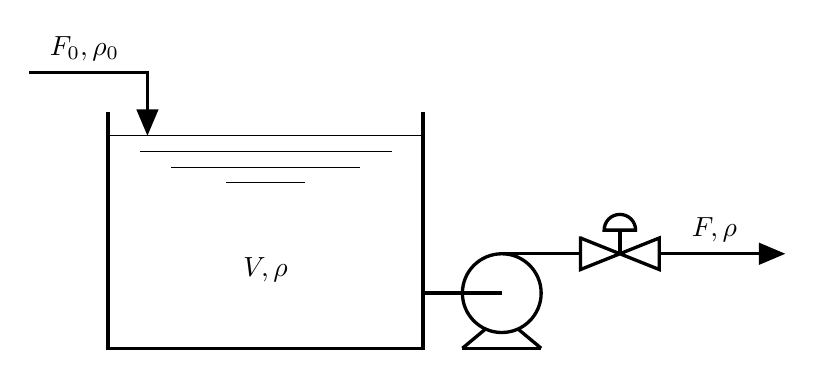
\begin{tikzpicture}[>=triangle 45]
%\draw[color=blue] (-2,-2) grid (11,11); %Tạo lưới
% Vẽ bình chứa
\drawe (0,3) -- (0,0) -- (4,0) -- (4,3);
\draw (0,2.7) -- (4,2.7);
\draw (0.4,2.5) -- (3.6, 2.5);
\draw (0.8,2.3) -- (3.2, 2.3);
\draw (1.5,2.1) -- (2.5, 2.1);
\draw (2,1) node {$V, \rho$};
\drawe(-1,3.5) -- (0.52,3.5);
\drawe[->] (0.5,3.5) -- (0.5,2.7);
\draw (-.3,3.8) node {$F_0,\rho_0$};
% Vẽ máy bơm
\drawe (4,.7) -- (5,.7);
\drawe (5,0.7) circle (.5);
\drawe (4.5,0) -- (5.5,0);
\drawe (4.5,0) -- (4.8,0.25);
\drawe (5.5,0) -- (5.2,0.25);
\drawe (5,1.2) -- (6,1.2);
\drawe (6,1.4) -- (7,1) -- (7,1.4) -- (6,1) -- (6,1.42);
\drawe (6.5,1.2) -- (6.5, 1.5);
\drawe (6.7,1.5) arc (0:180:.2) -- (6.72,1.5);
\drawe[->] (7,1.2) -- (8.6,1.2);
\draw (7.7,1.5) node {$F,\rho$};

\end{tikzpicture}
\end{document}